\documentclass[11pt]{article}
\usepackage[T1]{fontenc}
\usepackage[latin1]{inputenc}
\usepackage{enumerate}
\usepackage{setspace}
\usepackage{amsmath,amssymb,amsthm}
\usepackage{graphicx}
\usepackage{bbm}
\usepackage[round]{natbib}
\usepackage[nohead]{geometry}
\usepackage[bottom]{footmisc}
\usepackage{indentfirst}
\usepackage{endnotes}
\usepackage{graphicx}%
\usepackage{eurosym}
\usepackage{array}
\usepackage{booktabs}
\usepackage{caption}
\usepackage{subfig}
% \usepackage[hidelinks]{hyperref}
\usepackage{floatrow} %[capposition=top]
\floatsetup{footposition=bottom,capposition=top}
\renewcommand{\labelitemi}{--}
\renewcommand{\labelitemii}{$\bullet$}
\bibliographystyle{chicago}
% \geometry{left=1in,right=1in,top=1.00in,bottom=1.0in}
\let\olditemize\itemize
\renewcommand{\itemize}{
  \olditemize
  \setlength{\itemsep}{-1pt}
}

\begin{document}

\title{Creation of a low cost branch by a major retailer: Evidence from the French gasoline market\ \\ \ \\(Very preliminary)}
\author{Etienne Chamayou\thanks{e-mail:
\textit{etienne.chamayou@ensae.fr}}\medskip\\{\normalsize CREST and Department of Economics, Ecole Polytechnique }}
\maketitle

\sloppy%

\onehalfspacing

\textbf{Abstract:}

Total S.A is one of the five "supermajor" oil companies in the world and operates the largest gas station network in France. End of 2011, the company launched a new chain, "Total Access", with the stated goal of recapturing market shares lost due to the development of supermarket gas station chains. Within two years, 600 gas stations across France were thus rebranded to integrate the new chain, and for half of them the rebranding was accompanied by a sharp drop in prices. The creation of the brand and its impact on competition are studied using daily price data obtained from a comparison website. At an aggregate level, competitors' prices are found not to exhibit any significant adjustment. At an individidual level, upward adjustments are found to occur more frequently than price cuts. Such findings are consistent with a context of tough price competition imposed by supermarkets (limited ability to cut prices), and differentiation by other sellers in the market.

\strut

\textbf{Keywords:} Competition, Gasoline

\strut

\textbf{JEL Classification Numbers:} L13

\pagebreak%
%\doublespacing

\section{Introduction}

While supermarket chains only accounted for 12\% of retail gasoline sales in 1980, low price policies have allowed them to reach a current 60 \% market share. As a consequence, several traditional gas station operators have exited the markets (e.g. Shell, BP) or engaged in large divestment operations (e.g. Esso). On the other hand, the largest operator, Total, has decided end of 2011 to launch a new chain of gas stations characterized by a low price policy: "Total Access". Within two years, about 600 hundred gas stations were thus rebranded to integrate the new network. While half of them were previously operated under the chain "Elf" (inheritance from a merger) and already posted low prices, rebranding of the other c. 300 "Total" stations was accompanied by a sharp drop in prices.

Concerned about consumer information regarding gas station prices, the French governement has launched a comparison website in 2006. The creation of "Total Access" and the availability of a comprehensive price dataset on the period thus offer an interesting opportunity to assess the competitiveness of the French retail gasoline market.

The analysis is close to \cite{HAS04} which investigates the impact on competition of the purchase of a chain of independent gas stations by another operator in San Diego and Los Angeles in 1997. The rebranding of nearby a Total or Elf to Total Access is considered as a treatment for any non Total gas station. Daily price data at the gas station level allow to include time and station fixed effects so as to allow the identification of a potential pricing policy change. Regressions are run both at an aggregate level (pooling all stations, which, importantly, are treated at different dates) and at the gas station level with various control groups. The analysis is performed both with ex-Total gas stations, for which the rebranding is accompanied by a drop in price, and for ex-Elf gas stations, which are simply rebranded.

A large majority of gas station is found not to modify its pricing policy, and among reactions significantly more upward adjustments are observed than price cuts. A potential explanation is the fact that the rebranding induces more competition "at the bottom", where pricing was already quite aggressive, and less pressure "at the top".

\section{The French retail gasoline market}

The size of the French gas station network has been decreasing at a steady pace over the last decades, from c. 40,000 in 1980 to c. 12,000. Industry reports attribute this decline to two main causes: technological improvements affecting fuel consumption and the development of large supermarket gas stations with low price policies.

End of 2013, according to Nielsen, there were 11,476 gas stations in France, of which 4,979 were operated supermarkets. About 1,500 gas stations were reported to sell less than 500m$^{3}$, with the median gas station selling between 1,000 and 3,000m$^{3}$.

No chain implements a national or regional unique price policy. According to industry reports and interviews, only a small share of gas stations belonging to large retail chains decide prices. In general, chains have a team dedicated to pricing which uses information communicated by gas station managers about local competition to optimize prices.

Key cost components are the cost of wholesale gasoline, including delivery fees,  gas station operating expenses, and taxes. Taxes included a fix part called TICPE, which slightly varies across regions, and the classical Value-Added Tax (19.6\% over the period studied, which bear on cost and TICPE).

Regarding consumers, it is worth noticing that companies are offered card programs which allow them to monitor employees' consumptions and obtain rebates. An important implication is that the price actually paid may then not be the price posted at the gas station where fuel is obtained.

Consumers can get information about prices from a variety of sources including gps, mobile phone applications (e.g. Zagaz, Carbeo, Essence Free) or computer and mobile phone browser (Prix-Carburants.gouv.fr).

\section{Data}

\subsection{Data overview}

Data about daily diesel prices, gas station locations, opening hours and amenities were obtained from the governemental price  website prix-carburants.gouv.fr. The "Total Access" rebranding was found to be often declared with significant delay on the website as compared to a document from Total providing (non exhaustive) information about scheduled station renovations. While all ex "Total" gas stations could be fixed since the rebranding is accompanied by a sharp drop in prices, some uncertainty remains for ex "Elf" gas stations.

The period covered in the data starts on September 4, 2011 and ends on December 4, 2014. On some periods, prices could not be collected for various technical reasons, so that the maximum number of price observation for a gas station is 1,074. The database contains 10,231 gas stations, which is consistant with the number of gas station in France and the fact that small gas stations do not have to keep prices posted on the website).

\subsection{"Total Access"}

At the end of the period studied, there were 641 Total Access registered in the database, of which 374 were previously operated under the brand "Total" and 250 as "Elf" (others were either operated within another chain or information is missing). A map of the Total Access network end of 2014 is provided in Appendix. As can be observed in Figure \ref{fig:tot_price_distr}, prices of "Total" gas stations rebranded "Total Access" exhibit significant heterogeneity, reflecting the fact that they operate in very different market environments.

\begin{figure}
    \centering
    \subfloat[September 4, 2011]{{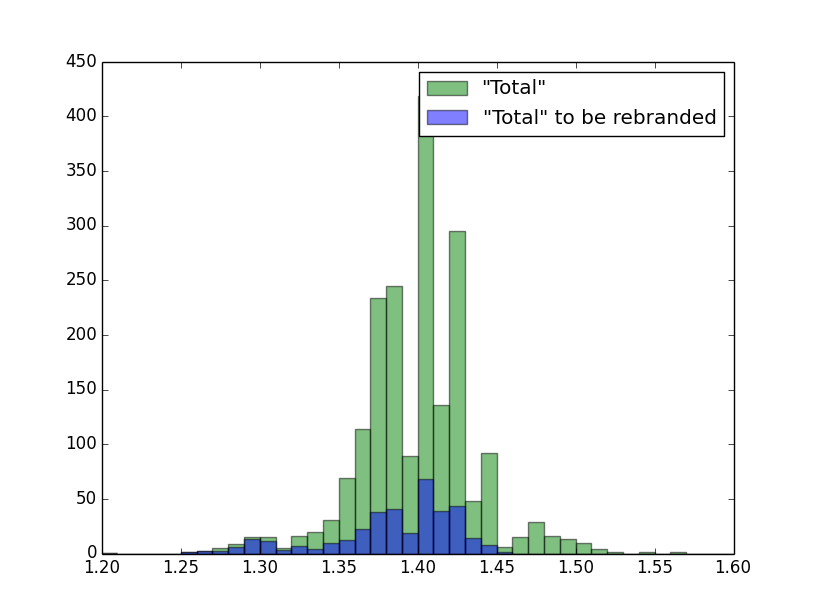
\includegraphics[width=7cm]{graphs/tot_pd_first.png}}}
    \qquad
    \subfloat[December 4, 2014]{{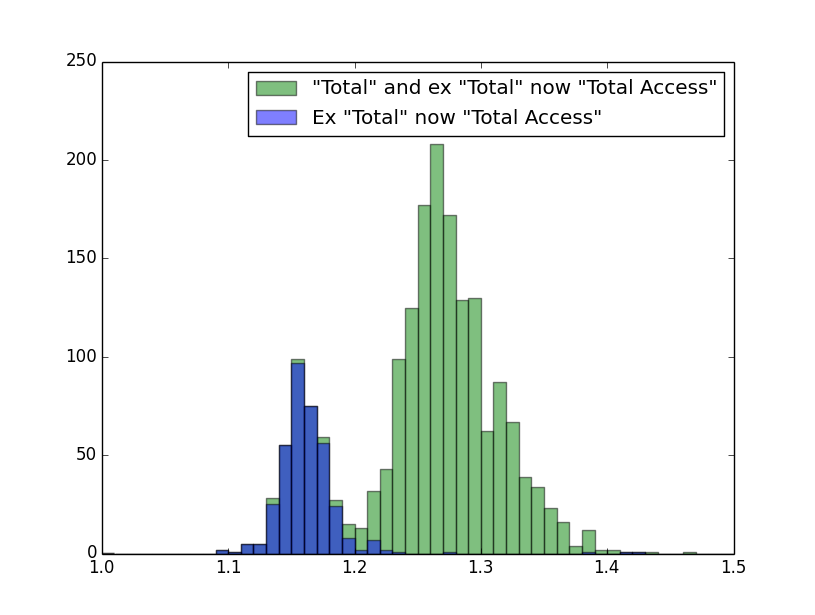
\includegraphics[width=7cm]{graphs/tot_pd_last.png}}}
    \caption{Total price distribution}
    \label{fig:tot_price_distr}
\end{figure}

For each rebranded station, a change in pricing policy was investigated by looking for the date which maximized the difference ( before and after the date) in estimated station fixed effect vs. the average national price. While no significant discontinuity could be identified for "Elf-Total Access" gas stations, it was the case for 344 "Total-Total Access" gas stations. An example is provided in Figure \ref{figure:rebranding_detection}.

\begin{figure}[H]
    \caption{Rebranding date detection}
	\centering
		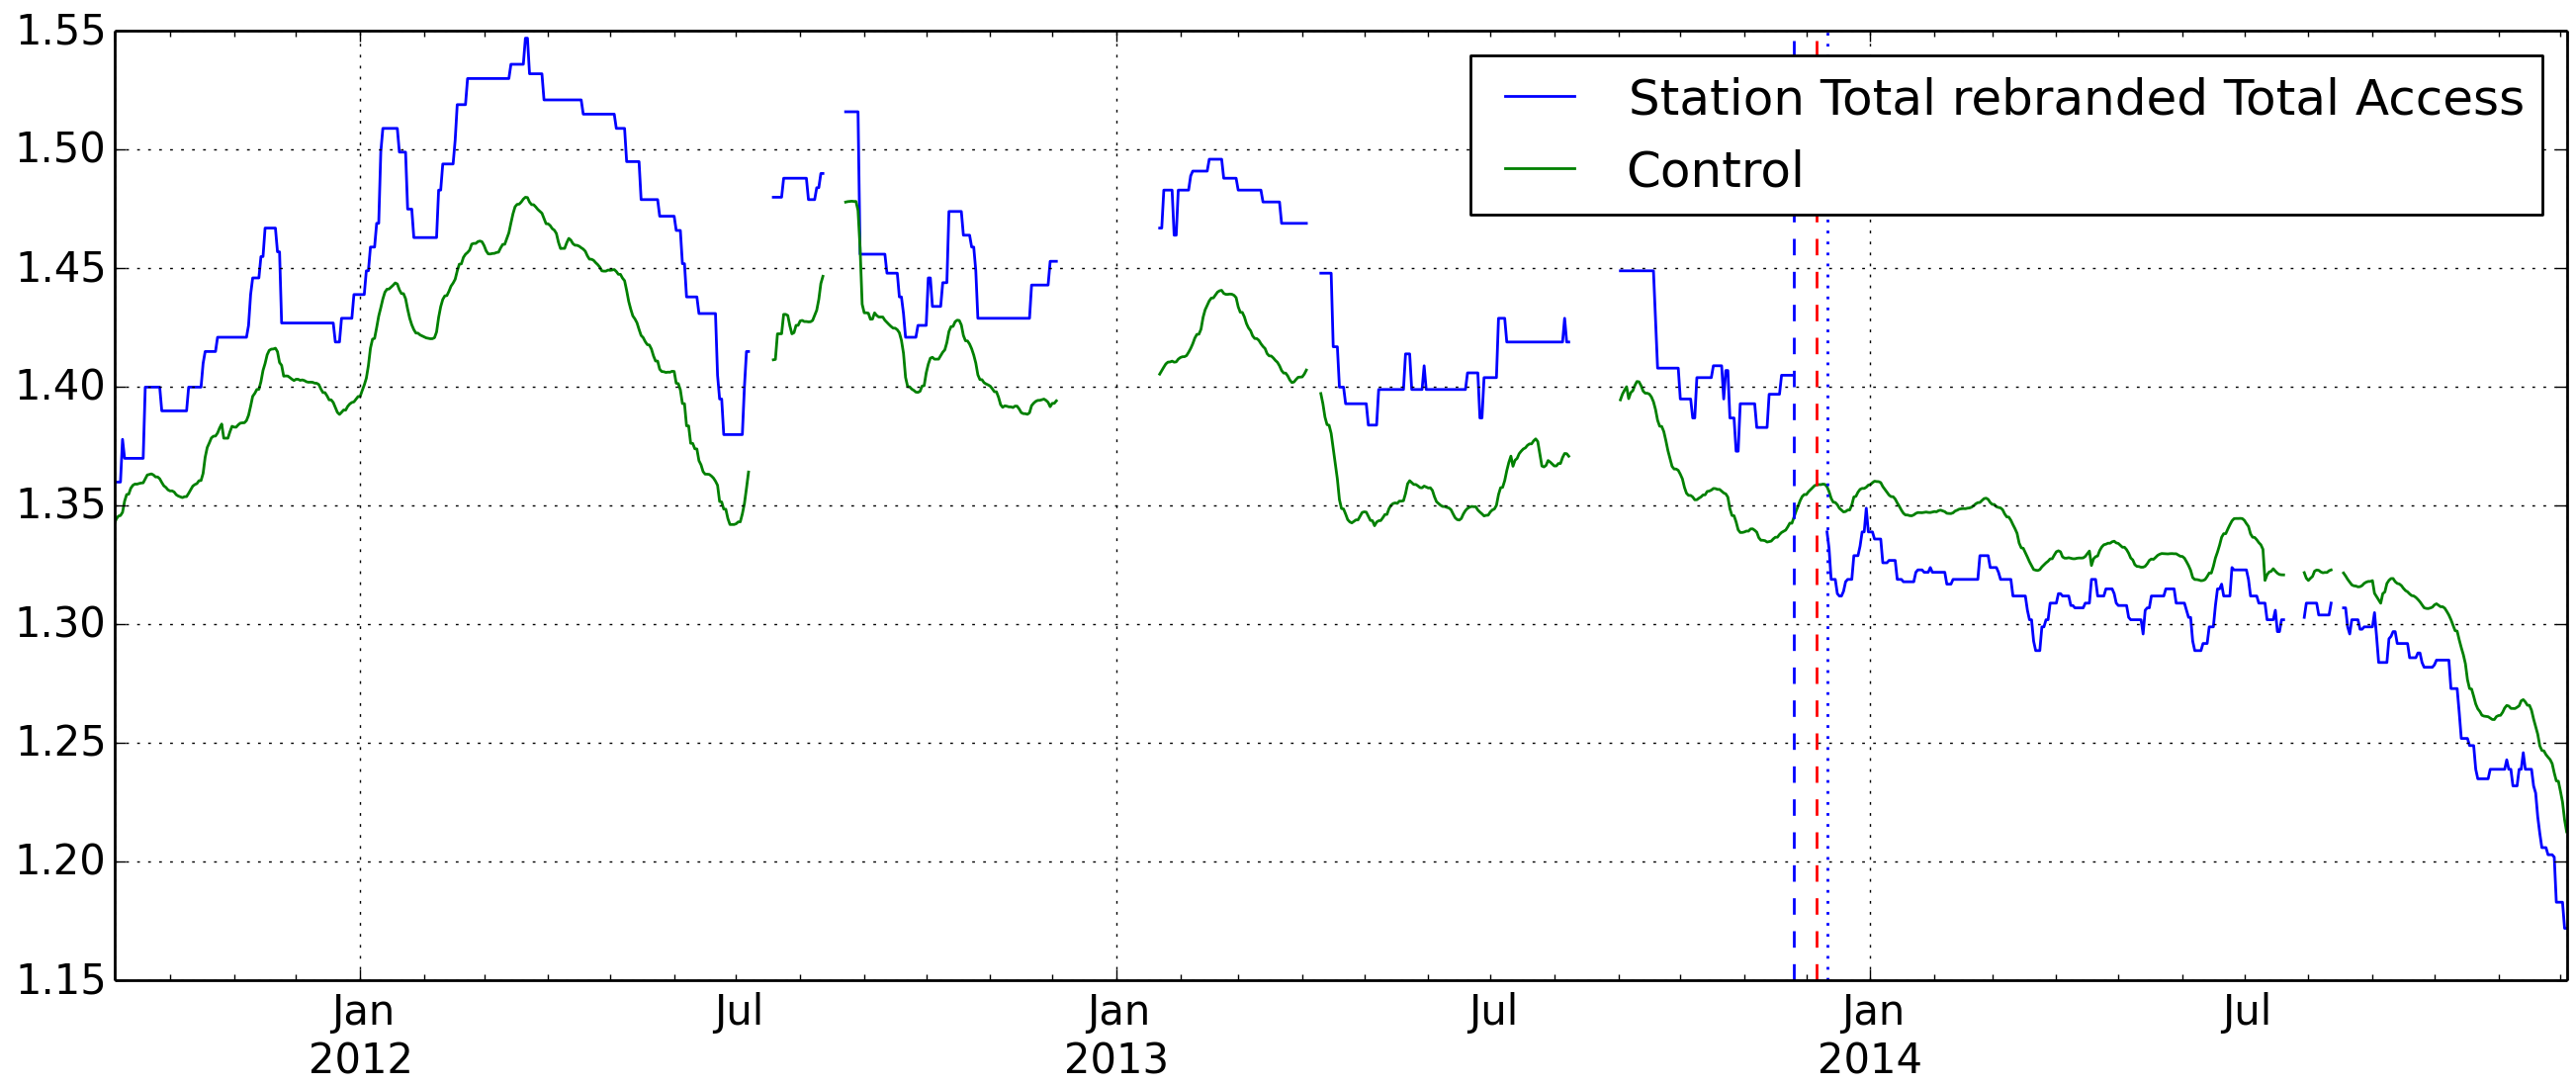
\includegraphics[width=15cm]{graphs/price_cut_detection_adj.png}
	\floatfoot{}
\label{figure:rebranding_detection}
\end{figure}

\subsection{Retail market definition}

In the following analysis, two stations are considered to be competitors whenever they are separated by a distance of less than 3 km (as the crow flies). In the analysis of the rebranding from "Total" to "Total Access", all stations which do not belong to the group Total and are located within 3 km of a Total-Total Access are considered as competitors. In the case of "Elf", on top of these conditions, it is imposed that no Total-Total Access is located within a radius of 10km. Indeed, with Elf-Total Access, the goal is to observe the impact of the rebranding without a price drop. Robustness checks were performed to ensure than findings were not sensitive to the radius used.

\section{Results}

\subsection{Aggregate fixed-effects estimation}

The richness of data allows to perform a regression with station-level fixed effects as well as day fixed-effects. The presence of station-level fixed effects is necessary given the differentiation observed between stations (location, brand image etc.), while day fixed-effects are included to account for variations in market conditions common to all gas stations. Since the rebranding occurs progressively over a period of two years, the regressions can be run by including stations of interest only (i.e. control is ensured by stations not yet affected by a rebranding and/or change in pricing policy).

\begin{align*}
p_{it} = \mu + \alpha_i + \delta_t + \theta r_{it} + \epsilon_{it}
\end{align*}
with $\mu$ a constant, $\alpha_i$ the station fixed-effects, $\delta_t$ the day fixed-effects, $r_{it}$ indicator equal to 1 in case of Rebranding. Table \ref{table:ta_fe_agg} reports the results of six regressions run according to this specification. In column (1), only the price of ex-Elf stations rebranded Total Access are included so that the Rebranding indicator captures the change in pricing policy implemented by Total. The same goes for column (4) with ex-Total stations rebranded Total. As expected, there is no significant change for ex-Elf stations (-0.1 cent), while the sharp drop in price for ex "Total" stations is appropriately captured with a nearly -10 cent estimated effect.

In columns (2) and (3), regressions are run with prices of competitors of Elf-Total Access gas stations. In column (3), the treatment is interacted with a categorical variable accounting for the "type" of the competitor: supermarket gas station, oil company gas station, or independent. A similar analysis is reported in columns (5) and (6) for competitors of Total-Total Access gas stations. Globally, reactions


\begin{table}[h]
\centering
\def\sym#1{\ifmmode^{#1}\else\(^{#1}\)\fi}
\caption{Aggregate FE estimates}
\begin{tabular}{lcccccc}
\toprule
\toprule
\multicolumn{7}{c}{Dependent variable:}\\
\multicolumn{7}{c}{Retail price for diesel (cents)}\\
\hline
{}                      & (1)                            & (2)                        & (3)                           & (4)                              & (5)                               & (6)                   \\
{}                      & Elf-TA                        & Elf-TA                    & Elf-TA                      & Total-TA                       & Total-TA                      & Total-TA                   \\
{}                      & station                      & competitors          & competitors             & station                        & competitors                & competitors              \\
\hline
Rebranding       & -0.140\sym{*}         & 0.036                    &                                 & -9.826\sym{***}       & -0.345\sym{***}      &                                  \\
                         & (0.067)                     & (0.128)                  &                                & (0.105)                       & (0.062)                      &                                  \\
\hline
Rebr. vs.           &                                  &                               & -0.329\sym{*}      &                                    &                                     & -0.634\sym{***}     \\
Supermarket     &                                  &                               & (0.139)                  &                                    &                                     & (0.066)                    \\
\hline
Rebr. vs.           &                                  &                               & 0.776\sym{**}      &                                    &                                   &  0.152                        \\
Oil company      &                                  &                                & (0.273)                 &                                    &                                    &  (0.131)                      \\
\hline
Rebr. vs.           &                                  &                               & 0.751                     &                                    &                                   & -0.079                      \\
Independent     &                                  &                               & (0.888)                  &                                    &                                    & (0.240)                     \\
\hline
Nb stations       & 250                           & 144                        & 144                         & 313                              & 604                            & 604                            \\
Obs                   & 257,600                    & 146,122                &  146,122                 & 322,273                      &  606,256                    & 606,256                     \\
R-square           & 0.910                        & 0.542                    &  0.581                     & 0.961                          &  0.588                        & 0.612                       \\
\hline\hline
\multicolumn{7}{l}{\footnotesize Standard errors in parentheses}\\
\multicolumn{7}{l}{\footnotesize \sym{*} \(p<0.05\), \sym{**} \(p<0.01\), \sym{***} \(p<0.001\)}\\
\end{tabular}
\floatfoot{All regressions are run with two way fixed effects for day and station. Standard errors are clustered at the station level}\\
\label{table:ta_fe_agg}
\end{table}

\subsection{Station level fixed-effect Estimation}

Results from aggregate analysis and observations suggest that there is significant heterogeneity in the reaction of stations competing with Total Access. In order to gain a better understanding of this heterogeneity, a similar analysis is performed at the gas station level. A treatment effect is now estimated for each gas station in a specific regression, where the control group is composed of stations operating in the same in the same "départment" (Metropolitan France is composed of 96 such regions) and not competing with a Total Access gas station.

The distribution of the treatment effects estimated for Elf-Total Access competitors is reported in Table \ref{table:ta_fe_indiv_elf}. While the overall effect is found to be slighly higher than at an aggregate level, results clearly establish that significant reactions are scarce.

\begin{table}[h]
\centering
\caption{Distribution of estimated individual treatment effects for Elfl-Total Access competitors (cents)}
\begin{tabular}{lrrrr}
\toprule
{} &     All &    Supermarket &    Oil company &     Independent \\
\midrule
count & 134 & 88 & 27 &  19 \\
mean  &   0.780 &  0.421 &  1.536 &   1.363 \\
std   &   1.764 &  0.944 &  1.551 &   3.656 \\
min   & -13.020 & -2.189 & -0.877 & -13.020 \\
10\%   &  -0.775 & -1.044 &  0.303 &   0.801 \\
25\%   &   0.280 &  0.158 &  0.569 &   1.177 \\
50\%   &   0.829 &  0.440 &  1.259 &   1.794 \\
75\%   &   1.386 &  0.983 &  1.906 &   2.818 \\
90\%   &   2.411 &  1.426 &  3.940 &   3.676 \\
max   &   5.778 &  2.420 &  5.778 &   4.200 \\
\bottomrule
\end{tabular}
\label{table:ta_fe_indiv_elf}
\end{table}

In Table \ref{table:ta_fe_indiv_tta}, the distribution of the treatment effects estimated for Total-Total Access competitors is reported. Remarkably, the distribution is quite similar to the distribution for Elf-Total Access. Supermarkets are found to be more likely to have decreased prices than oil company and independent gas stations. As compared to the average c.10 cent price cut estimated at over 300. Total-Total Access gas stations, only 38 competitors are found to have cut price by more than 2 cents, of which 25 supermarkets. On the other hand, 163 gas stations are found to have increased prices by more than 2 cents, of which 103 oil company gas stations.

\begin{table}[h]
\centering
\caption{Distribution of estimated individual treatment effects for Total-Total Access competitors (cents)}
\begin{tabular}{lrrrr}
\toprule
{} &     All &    Supermarket &    Oil company &     Independent \\
\midrule
count & 956 & 572 & 276 & 108 \\
mean  &   0.782 &   0.421 &   1.421 &   1.064 \\
std   &   1.512 &   1.183 &   1.617 &   2.095 \\
min   &  -6.824 &  -4.088 &  -6.824 &  -5.985 \\
10\%   &  -0.907 &  -1.007 &  -0.521 &  -1.272 \\
25\%   &   0.174 &  -0.232 &   0.486 &   0.192 \\
50\%   &   0.746 &   0.522 &   1.558 &   1.219 \\
75\%   &   1.628 &   1.072 &   2.536 &   1.906 \\
90\%   &   2.543 &   1.675 &   3.231 &   3.049 \\
max   &  11.738 &   4.890 &   5.769 &  11.738 \\
\bottomrule
\end{tabular}
\label{table:ta_fe_indiv_tta}
\end{table}

\clearpage

\section{Conclusion}

The creation of the chain "Total Access" offers the opportunity to study the impact on many local markets of a unilateral sharp decrease in price. Empirical results suggest that a large majority of affected competitors has not changed its price policy, and that upward adjustments were more frequent that price cuts. Such findings are consistent with tough price competition between supermarkets and differentiation from oil company and independent gas stations.

\clearpage

\bibliography{references}

\newpage

\appendix

\section{Maps}

\begin{figure}[H]
	\centering
		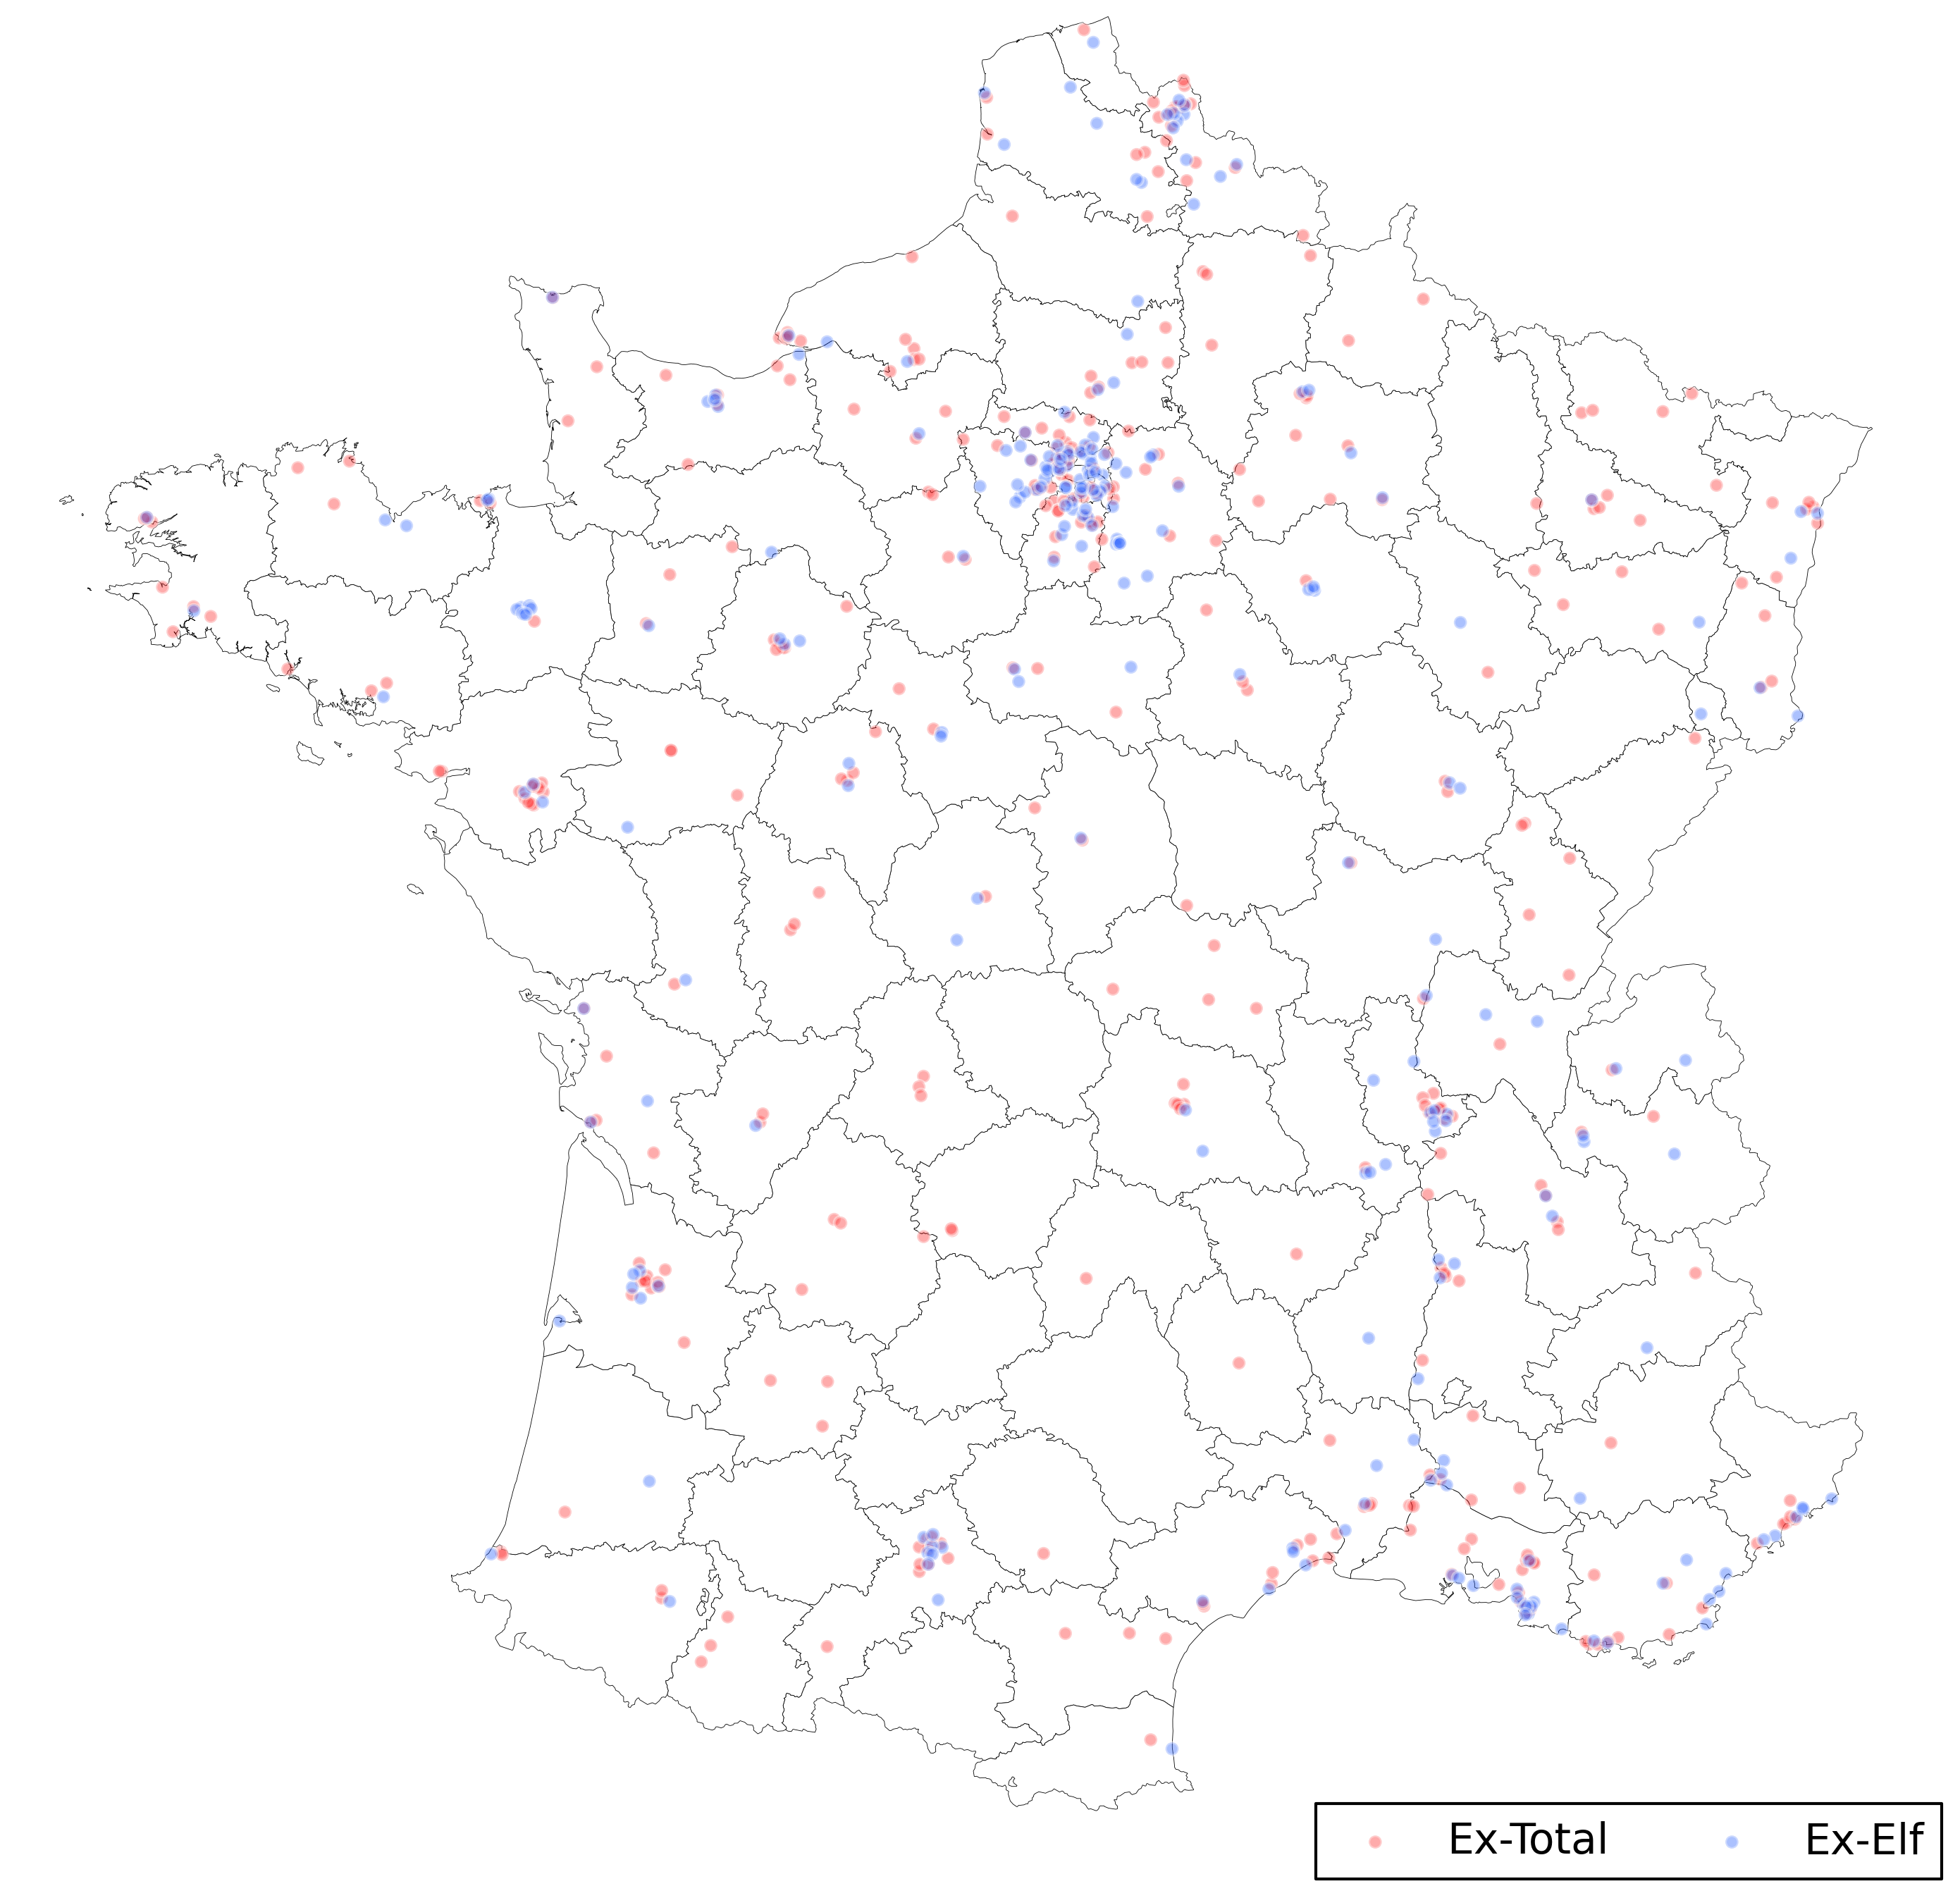
\includegraphics[width=16cm]{graphs/map_ta_adj.png}
	\floatfoot{}
\caption{Total Access gas stations end 2014}
\label{figure:map_ta}
\end{figure}

\section{Price trends: Total stations rebranded Total Access}

\begin{figure}[H]
    \centering
    \subfloat[Before rebranding (2011-2012)]{{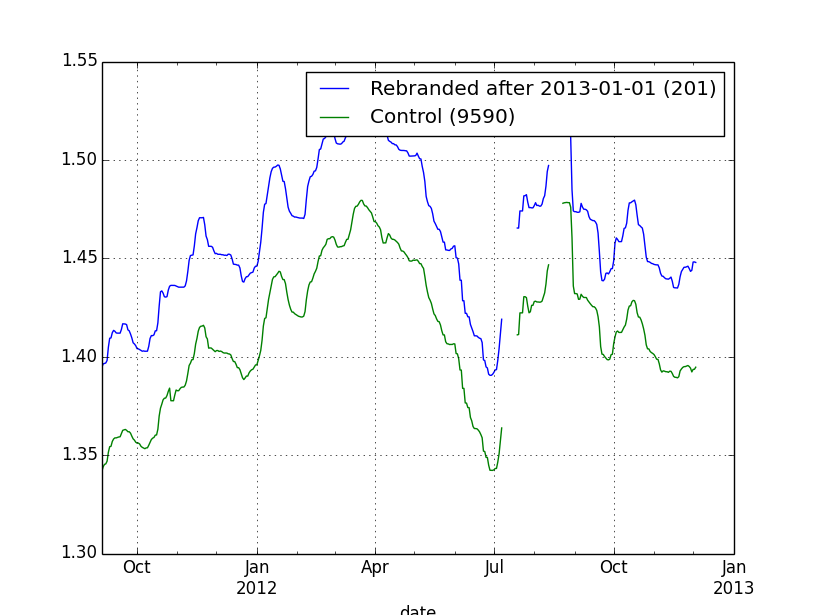
\includegraphics[width=7cm]{graphs/not_yet_rebranded_2013.png}}}
    \qquad
    \subfloat[Before rebranding (2011-2013)]{{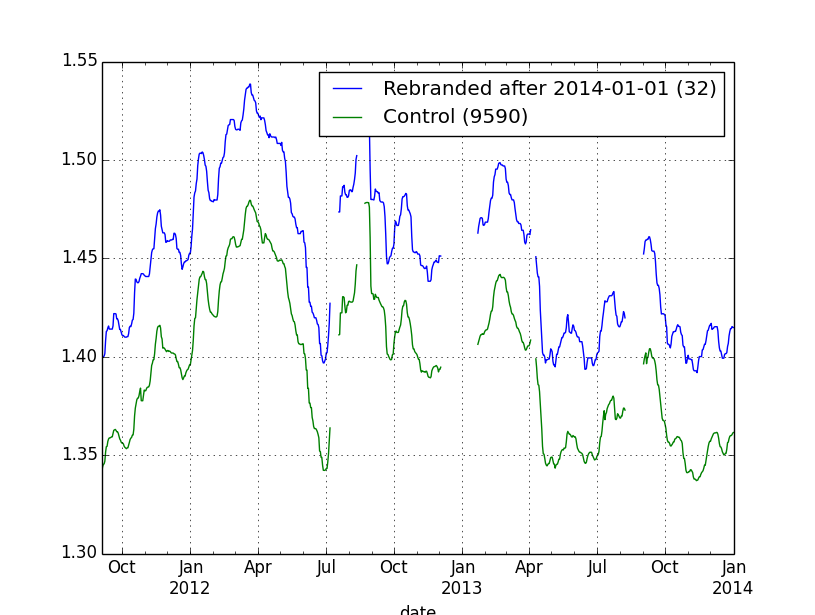
\includegraphics[width=7cm]{graphs/not_yet_rebranded_2014.png}}}
    \caption{Average price of Total stations to be rebranded vs. national price (number of stations in parenthesis)}
    \label{fig:not_yet}
\end{figure}

\begin{figure}[H]
    \centering
    \subfloat[After rebranding (2013-2014)]{{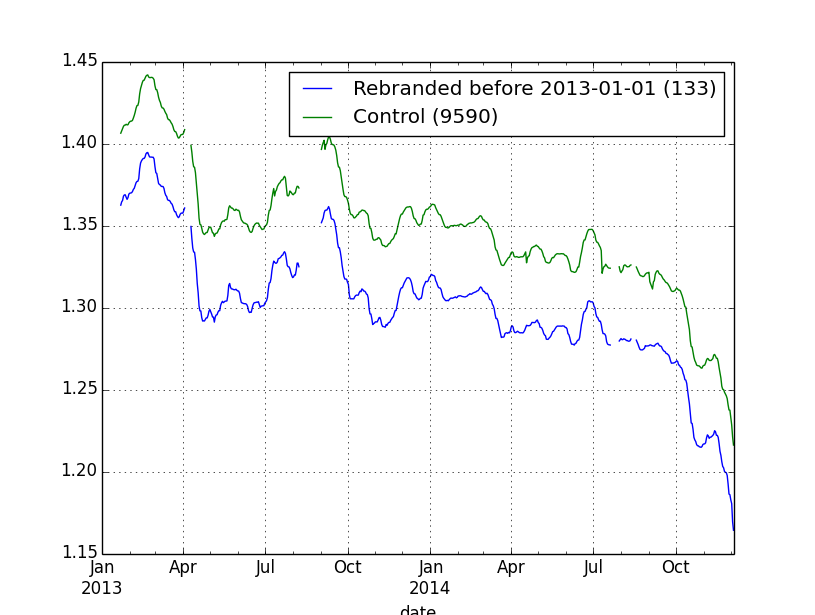
\includegraphics[width=7cm]{graphs/rebranded_before_2013.png}}}
    \qquad
    \subfloat[After rebranding (2014)]{{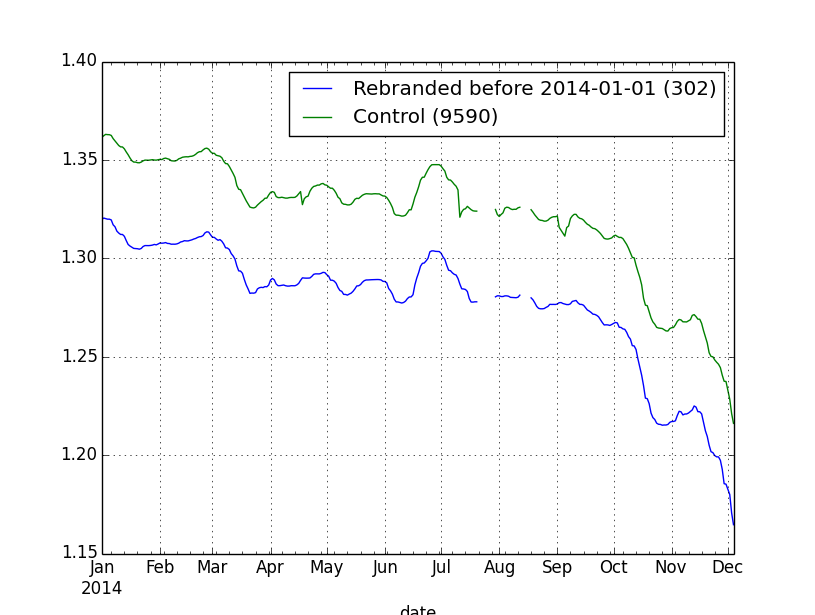
\includegraphics[width=7cm]{graphs/rebranded_before_2014.png}}}
    \caption{Average price of ex Total now Total Access vs.national price (number of stations in parenthesis)}
    \label{fig:rebranded_before}
\end{figure}

\section{Price trends: Elf stations rebranded Total Access}

\begin{figure}[H]
	\centering
		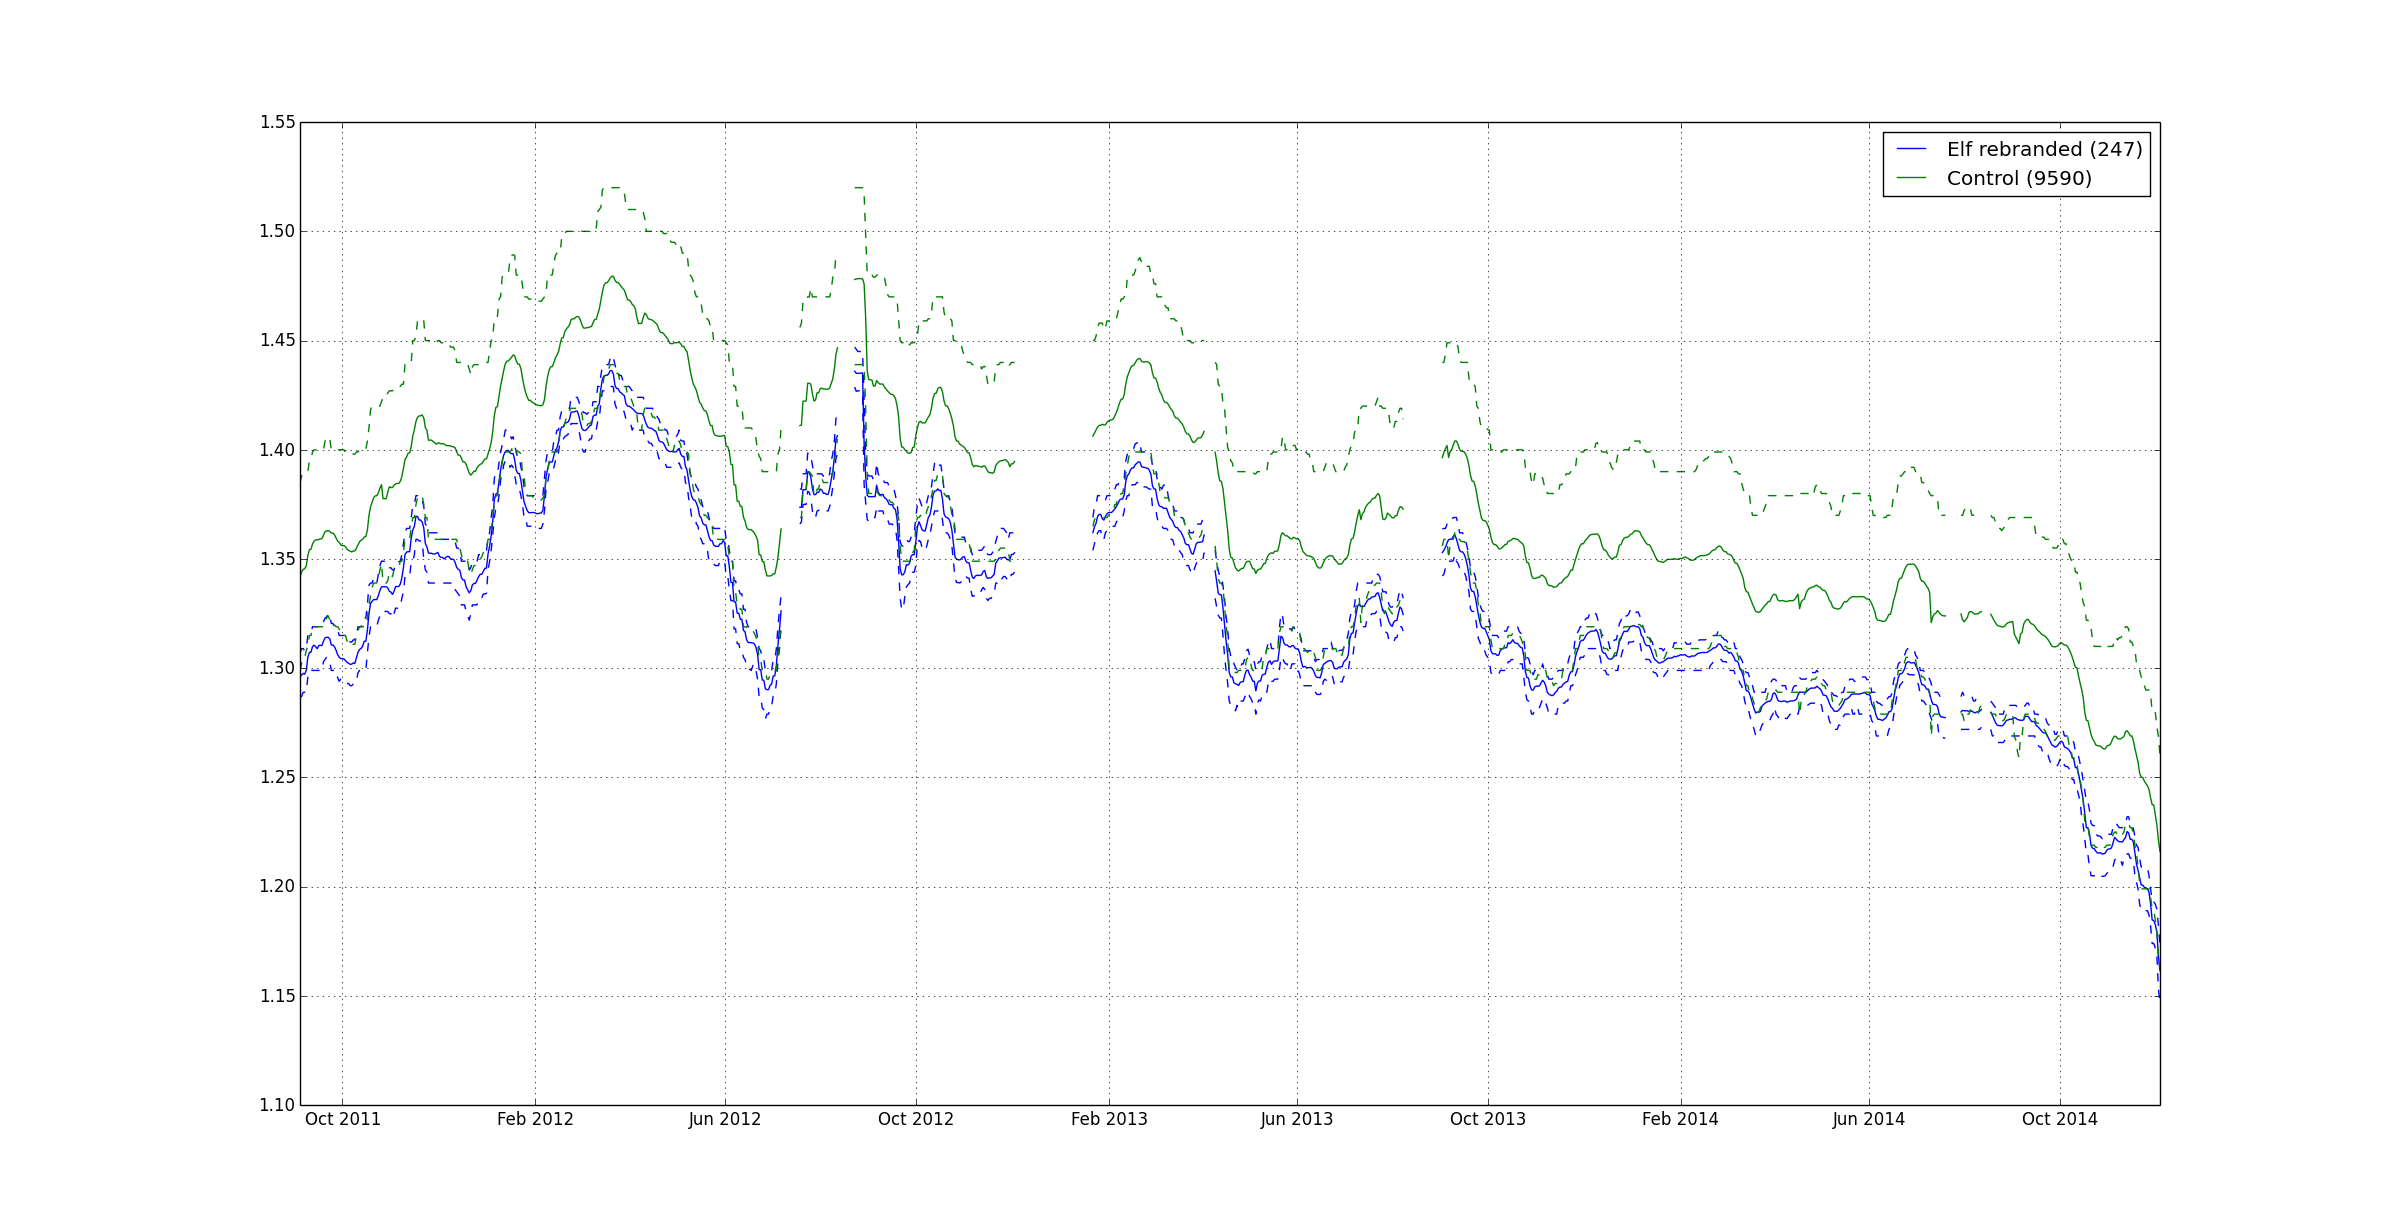
\includegraphics[width=17cm]{graphs/elf_trend.png}
	\floatfoot{}
\caption{Average Elf - Total Access station prices vs. national price}
\label{figure:elf_prices}
\end{figure}

\section{Competitor reactions: examples}

\begin{figure}[H]
	\centering
		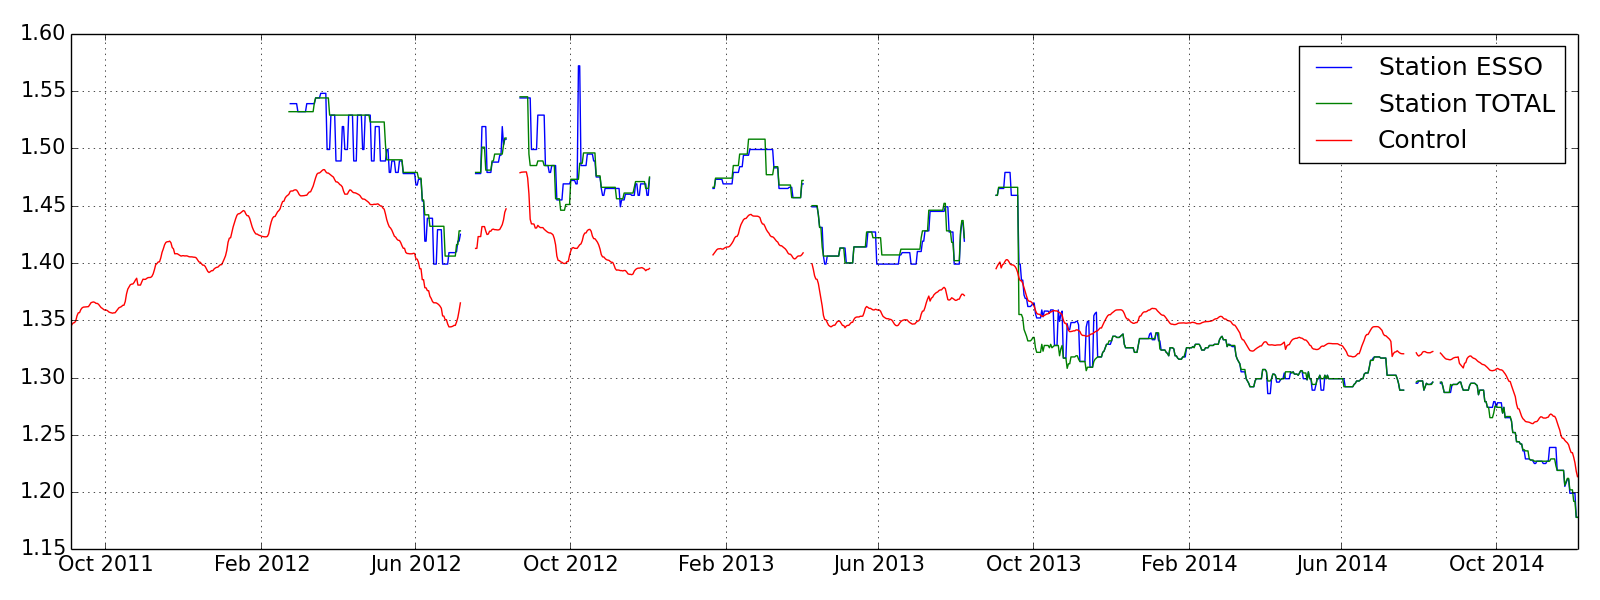
\includegraphics[width=16cm]{graphs/ex_0.png}
	\floatfoot{}
\caption{Competition with an oil company gas station}
\label{figure:fierce_competition}
\end{figure}

\begin{figure}[H]
	\centering
		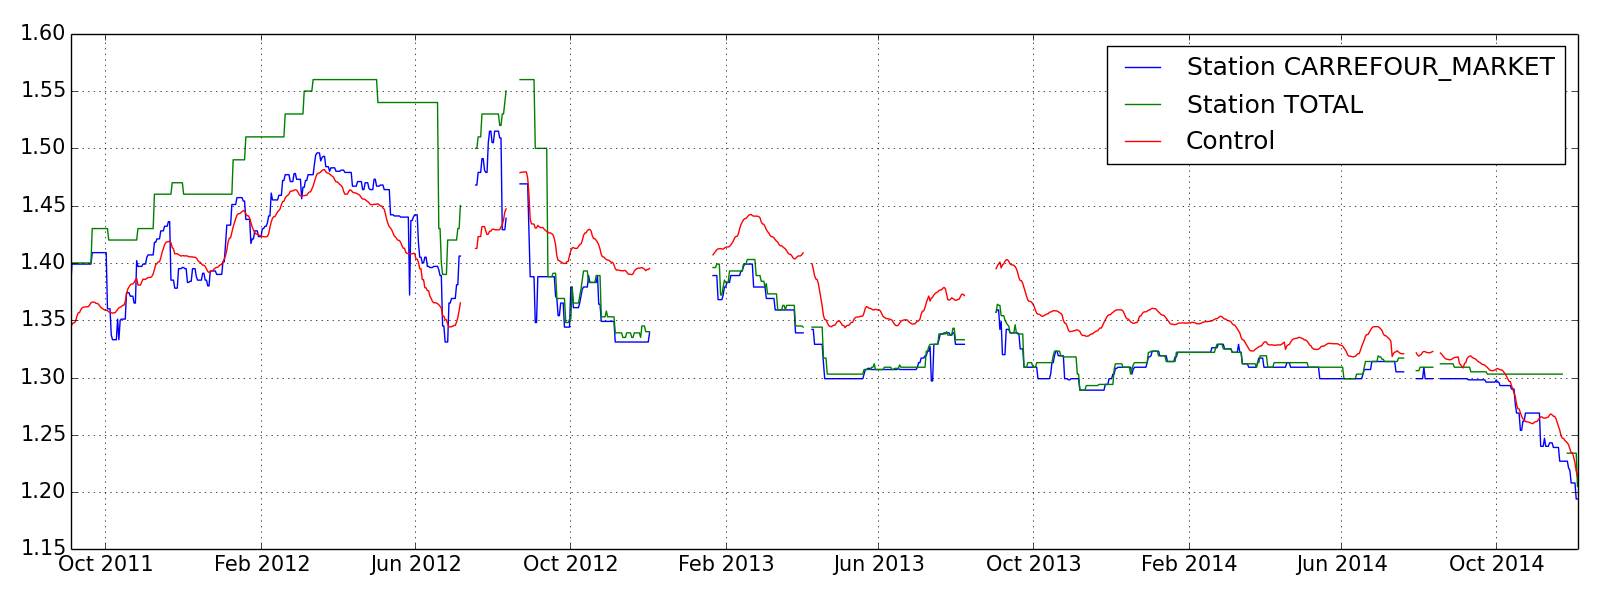
\includegraphics[width=16cm]{graphs/ex_2.png}
	\floatfoot{}
\caption{Competition with a supermarket}
\label{figure:given_up}
\end{figure}

\begin{figure}[H]
	\centering
		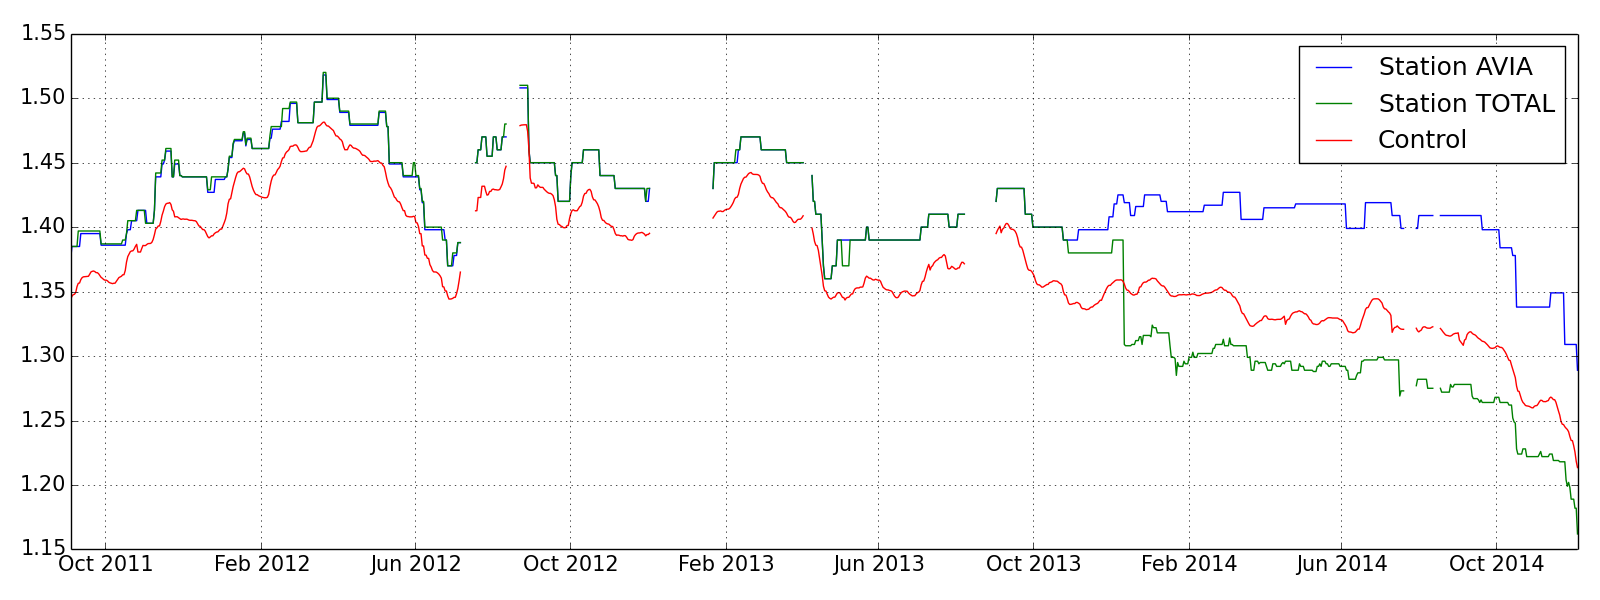
\includegraphics[width=16cm]{graphs/ex_3.png}
	\floatfoot{}
\caption{Increase in price 1}
\label{figure:given_up}
\end{figure}

\begin{figure}[H]
	\centering
		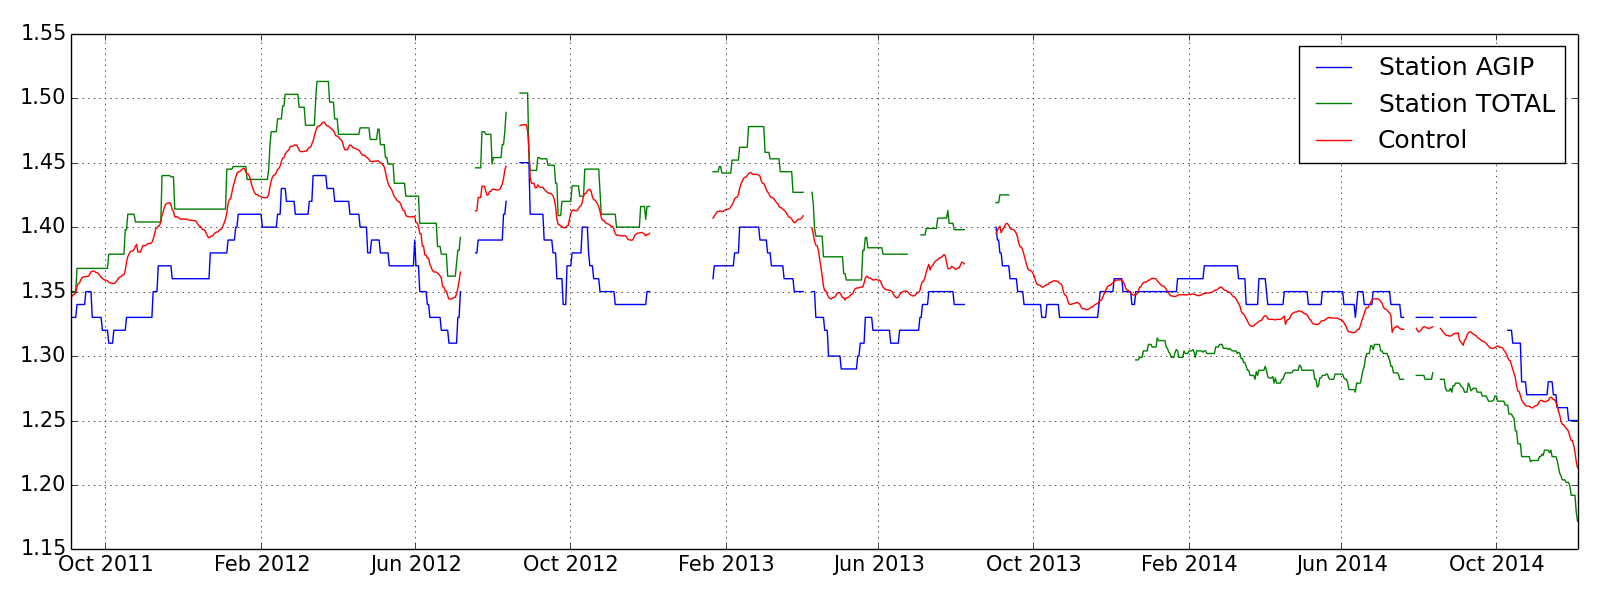
\includegraphics[width=16cm]{graphs/ex_4.png}
	\floatfoot{}
\caption{Increase in price 2}
\label{figure:given_up}
\end{figure}

\end{document} 